\documentclass[11pt]{article}
\pdfoutput=1

\usepackage{../../jcapmod}
\input{../../preamble}
\graphicspath{{figures/}}

% TikZ for inline figures
\usetikzlibrary{positioning, arrows.meta, shapes.geometric, fit, backgrounds, matrix, decorations.pathreplacing}

% For boxed content
\usepackage{tcolorbox}

% Bibliography
\usepackage[numbers,sort&compress]{natbib}
\bibliographystyle{unsrtnat}

\begin{document}
\thispagestyle{plain}

\newcommand{\eqicon}{%
\raisebox{-0.12ex}{
\begin{tikzpicture}[scale=1.2]
    % Rotation arrow symbol
    \draw[line width=0.7pt, ->] (0.15, 0) arc (0:300:0.15);
    \fill (0, 0) circle (1pt);
\end{tikzpicture}}%
}

\chapterheading{\eqicon\hspace{0.4em}$\cdot$ Symmetry-Preserving Neural Networks}

\vspace{1em}
\begin{quote}
\textit{``A molecule does not concern itself with the orientation of the coordinate axes.''}
\end{quote}
\vspace{0.5em}

\section{Symmetry in physical systems}

A molecule's energy doesn't change if you rotate it or translate it through space. These are \emph{symmetries}: transformations that leave physical quantities unchanged. In the previous chapter, we saw how CNNs encode translation symmetry and GNNs encode permutation symmetry. Physical systems often have additional continuous symmetries---rotations, translations, reflections---that we can build into neural network architectures.

%%%%%%%%%%%%%%%%%%%%%%%%%%%%%%%%%%%%%%%%%%%%%%%%%%%%%%%%%%%%%%%%%%
\section{Invariance and equivariance}
%%%%%%%%%%%%%%%%%%%%%%%%%%%%%%%%%%%%%%%%%%%%%%%%%%%%%%%%%%%%%%%%%%

When we apply a symmetry transformation to the input, the output can respond in two fundamentally different ways.

\paragraph{Invariance.} An \emph{invariant} function produces the same output regardless of how the input is transformed:
\beq
f(g \cdot x) = f(x)
\eeq
Energy is the canonical example. Rotate a molecule by any angle, translate it anywhere in space---the energy stays exactly the same. The function ``doesn't see'' the transformation.

\paragraph{Equivariance.} An \emph{equivariant} function has outputs that transform consistently with the inputs:
\beq
f(g \cdot x) = g \cdot f(x)
\eeq
Forces are equivariant. Rotate a molecule, and the force vectors rotate with it. The force on atom $i$ still points in the same direction \emph{relative to the molecule}---but in the lab frame, it has rotated along with everything else. The function ``sees'' the transformation and responds accordingly.

The distinction matters for what you're predicting. Scalar quantities---energy, charge, mass, binding affinity---should be invariant. Vector quantities---forces, velocities, dipole moments---should be equivariant. Per-atom outputs that describe spatial relationships (like predicted displacements) should be equivariant.

\begin{figure}[h]
\centering
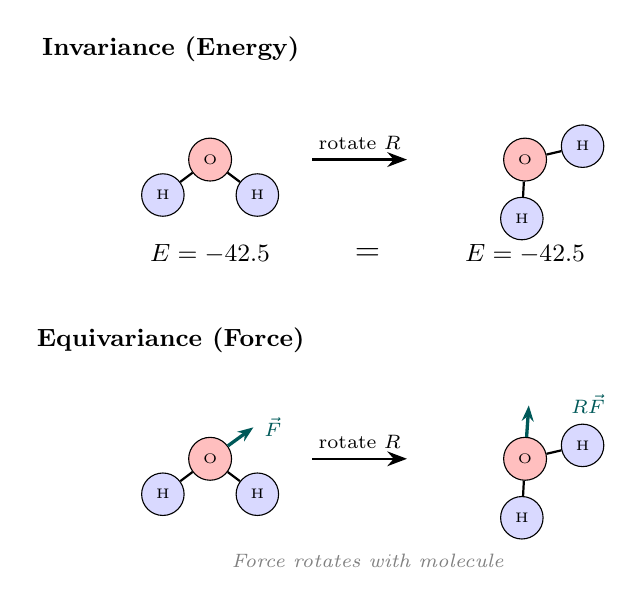
\begin{tikzpicture}[
    atom/.style={circle, draw, fill=blue!20, minimum size=0.35cm, font=\tiny},
    atomO/.style={atom, fill=red!25},
    atomH/.style={atom, fill=blue!15},
    arrow/.style={-{Stealth[length=2.5mm]}, thick},
    force/.style={-{Stealth[length=2mm]}, very thick, teal!70!black},
    label/.style={font=\small}
]

% === INVARIANCE (TOP) ===
\node[font=\small\bfseries] at (-0.5, 3.2) {Invariance (Energy)};

% Original molecule
\begin{scope}[shift={(0, 1.8)}]
    \node[atomO] (O1) at (0, 0) {\tiny O};
    \node[atomH] (H1a) at (-0.6, -0.45) {\tiny H};
    \node[atomH] (H1b) at (0.6, -0.45) {\tiny H};
    \draw[thick] (O1) -- (H1a);
    \draw[thick] (O1) -- (H1b);
\end{scope}

% Arrow
\draw[arrow] (1.3, 1.8) -- node[above, font=\scriptsize] {rotate $R$} (2.5, 1.8);

% Rotated molecule
\begin{scope}[shift={(4, 1.8)}, rotate=50]
    \node[atomO] (O2) at (0, 0) {\tiny O};
    \node[atomH] (H2a) at (-0.6, -0.45) {\tiny H};
    \node[atomH] (H2b) at (0.6, -0.45) {\tiny H};
    \draw[thick] (O2) -- (H2a);
    \draw[thick] (O2) -- (H2b);
\end{scope}

% Energy outputs
\node[font=\small] at (0, 0.6) {$E = -42.5$};
\node[font=\small] at (4, 0.6) {$E = -42.5$};
\node[font=\large] at (2, 0.6) {$=$};

% === EQUIVARIANCE (BOTTOM) ===
\node[font=\small\bfseries] at (-0.5, -0.5) {Equivariance (Force)};

% Original molecule with force
\begin{scope}[shift={(0, -2)}]
    \node[atomO] (O3) at (0, 0) {\tiny O};
    \node[atomH] (H3a) at (-0.6, -0.45) {\tiny H};
    \node[atomH] (H3b) at (0.6, -0.45) {\tiny H};
    \draw[thick] (O3) -- (H3a);
    \draw[thick] (O3) -- (H3b);
    \draw[force] (O3) -- ++(0.55, 0.4) node[right, font=\scriptsize] {$\vec{F}$};
\end{scope}

% Arrow
\draw[arrow] (1.3, -2) -- node[above, font=\scriptsize] {rotate $R$} (2.5, -2);

% Rotated molecule with rotated force
\begin{scope}[shift={(4, -2)}, rotate=50]
    \node[atomO] (O4) at (0, 0) {\tiny O};
    \node[atomH] (H4a) at (-0.6, -0.45) {\tiny H};
    \node[atomH] (H4b) at (0.6, -0.45) {\tiny H};
    \draw[thick] (O4) -- (H4a);
    \draw[thick] (O4) -- (H4b);
    \draw[force] (O4) -- ++(0.55, 0.4);
\end{scope}
\node[font=\scriptsize, teal!70!black] at (4.8, -1.3) {$R\vec{F}$};

% Annotation
\node[font=\scriptsize\itshape, text=gray] at (2, -3.3) {Force rotates with molecule};

\end{tikzpicture}

\caption{Invariance vs.\ equivariance. (Top) Energy is invariant: rotating the molecule doesn't change its energy. (Bottom) Force is equivariant: rotating the molecule rotates the force vectors.}
\label{fig:inv_equiv}
\end{figure}

%%%%%%%%%%%%%%%%%%%%%%%%%%%%%%%%%%%%%%%%%%%%%%%%%%%%%%%%%%%%%%%%%%
\section{Building in translation invariance}
%%%%%%%%%%%%%%%%%%%%%%%%%%%%%%%%%%%%%%%%%%%%%%%%%%%%%%%%%%%%%%%%%%

Translation invariance is the easiest symmetry to encode: \textbf{never use absolute positions}.

If your input is atom positions $\{r_i\}$, don't feed raw coordinates into the network. Instead, use quantities that are intrinsically translation-invariant: \emph{relative positions} $r_{ij} = r_i - r_j$ between pairs of atoms, or \emph{distances} $d_{ij} = \|r_i - r_j\|$. Shift all atoms by the same vector, and these quantities don't change---the relative geometry is preserved.

This simple prescription eliminates an entire class of failure modes. Networks trained on absolute positions can learn arbitrary correlations with the coordinate system, e.g. ``molecules centered at the origin have property X.''. These patterns may hold in the training set (if all molecules happen to be centered) but reflect no physics. By using only relative quantities, we make such spurious patterns impossible to learn.

%%%%%%%%%%%%%%%%%%%%%%%%%%%%%%%%%%%%%%%%%%%%%%%%%%%%%%%%%%%%%%%%%%
\section{Invariant networks: the simplest approach}
%%%%%%%%%%%%%%%%%%%%%%%%%%%%%%%%%%%%%%%%%%%%%%%%%%%%%%%%%%%%%%%%%%

The simplest way to achieve rotation invariance: \textbf{only use distances}. Distances $d_{ij} = \|x_i - x_j\|$ don't change under rotation. If your network only sees distances (never positions or relative vectors), it's automatically invariant.

\paragraph{SchNet-style architecture.} Recall message passing from the previous chapter: each node $i$ in a graph updates its features by aggregating information from neighbors $j \in \mathcal{N}(i)$. SchNet~\cite{schutt2017schnet} makes this rotation-invariant by having messages depend only on distances:
\beq
h_i' = h_i + \sum_{j \in \mathcal{N}(i)} \phi(h_j) \cdot w(d_{ij})
\eeq
Each neighbor $j$ sends a message $\phi(h_j)$ weighted by a learned function of distance $w(d_{ij})$. The network never sees coordinates directly---only pairwise distances. This guarantees rotation and translation invariance.

\begin{figure}[h]
\centering
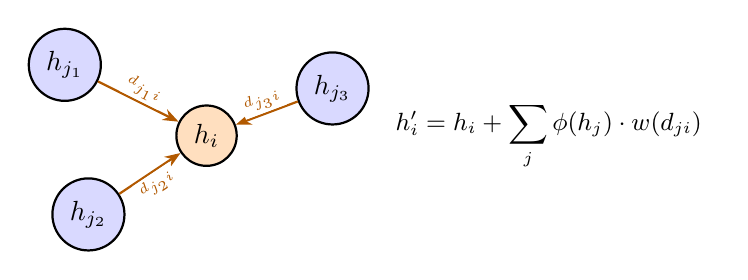
\begin{tikzpicture}[
    node distance=1.2cm,
    atom/.style={circle, draw, minimum size=0.75cm, thick, fill=blue!15},
    target/.style={atom, fill=orange!25},
    msg/.style={-{Stealth[length=2mm]}, thick, orange!70!black},
    dist/.style={font=\tiny, fill=white, inner sep=1pt},
    label/.style={font=\scriptsize}
]

% Central atom (target)
\node[target] (i) at (0, 0) {$h_i$};

% Neighbors
\node[atom] (j1) at (-1.8, 0.9) {$h_{j_1}$};
\node[atom] (j2) at (-1.5, -1.0) {$h_{j_2}$};
\node[atom] (j3) at (1.6, 0.6) {$h_{j_3}$};

% Distance labels and message arrows
\draw[msg] (j1) -- node[dist, above, sloped] {$d_{j_1 i}$} (i);
\draw[msg] (j2) -- node[dist, below, sloped] {$d_{j_2 i}$} (i);
\draw[msg] (j3) -- node[dist, above, sloped] {$d_{j_3 i}$} (i);


% Update equation on right
\node[font=\small, align=left] at (4.4, 0) {
$h_i' = h_i + \displaystyle\sum_{j} \phi(h_j) \cdot w(d_{ji})$
};

\end{tikzpicture}

\caption{SchNet-style invariant message passing. Each neighbor sends a message weighted by a learned function of distance $w(d_{ji})$. The network only sees distances, never positions, ensuring rotation and translation invariance.}
\label{fig:schnet}
\end{figure}

\paragraph{Encoding distances.} How should $w(d_{ij})$ depend on distance? A neural network needs a good representation of the scalar $d_{ij}$. The standard approach: \emph{radial basis functions}.

Expand the distance into a set of basis functions, typically Gaussians centered at different values:
\beq
e_k(d) = \exp\left( -\gamma (d - \mu_k)^2 \right)
\eeq
with centers $\mu_k$ spaced from 0 to some cutoff (e.g., $\mu_k = 0, 0.5, 1.0, \ldots, 5.0$ \AA). This gives a vector $[e_1(d), e_2(d), \ldots, e_K(d)]$ that the network can process with standard linear layers.

Why not just use $d$ directly? A single scalar gives the network little to work with. The basis expansion provides a richer representation: each basis function ``activates'' for distances near its center, giving the network easy access to distance information at different scales.

\begin{figure}[h]
\centering
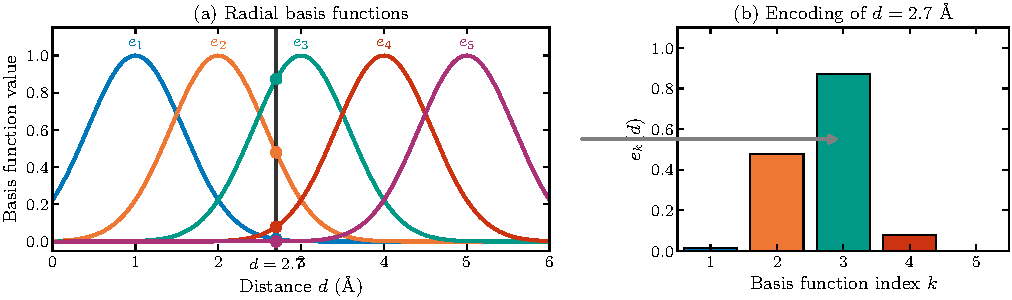
\includegraphics[width=\textwidth]{../03-neural-networks/figures/radial_basis_functions.pdf}
\caption{Radial basis function encoding. (a) Five Gaussians centered at different distances. A vertical line marks an example distance $d = 2.7$\,\AA; dots show where it intersects each basis function. (b) The resulting encoding: a 5-dimensional vector where each entry is one basis function's activation. One scalar (distance) becomes a vector the network can process.}
\label{fig:rbf}
\end{figure}

\paragraph{Cutoff functions.} Atoms far apart don't interact much. For efficiency (and physics), we restrict to neighbors within a cutoff radius $r_c$:
\beq
\tilde{w}(d) = w(d) \cdot f_{\text{cut}}(d)
\eeq
where $f_{\text{cut}}(d)$ smoothly goes to zero as $d \to r_c$. A common choice:
\beq
f_{\text{cut}}(d) = \begin{cases}
\frac{1}{2}\left[\cos\left(\frac{\pi d}{r_c}\right) + 1\right] & d < r_c \\
0 & d \geq r_c
\end{cases}
\eeq
Smooth cutoffs matter: discontinuities in the energy would cause infinite forces.

%%%%%%%%%%%%%%%%%%%%%%%%%%%%%%%%%%%%%%%%%%%%%%%%%%%%%%%%%%%%%%%%%%
\section{Equivariant networks: when you need vectors}
%%%%%%%%%%%%%%%%%%%%%%%%%%%%%%%%%%%%%%%%%%%%%%%%%%%%%%%%%%%%%%%%%%

Invariant networks predict scalars. But what if you need \emph{vector} outputs---forces, velocities, dipole moments? These should rotate with the input, and in this case we need to encode \emph{equivariance}.

\paragraph{Scalar and vector features.} The key idea is to maintain two types of features at each node: \emph{scalar features} $h_i \in \R^d$ that are invariant to rotation, and \emph{vector features} $\vec{v}_i \in \R^{3 \times d}$ that rotate with the input.

How can we combine these without breaking equivariance? Scalars are flexible---you can add them, multiply them, pass them through any nonlinearity you like. Vectors are more constrained: you can add vectors and scale them by scalars, but you \emph{cannot} pass them through elementwise nonlinearities like ReLU. Applying $\text{ReLU}(v_x, v_y, v_z)$ component-wise would break rotation equivariance---the result depends on how the coordinate axes are oriented.

The allowed operations form an algebra: inner products of vectors produce scalars (the dot product is rotation-invariant), and scalars times vectors produce vectors (scaling doesn't break equivariance). These constraints may seem limiting, but they're enough to build powerful architectures.

\paragraph{The EGNN approach.} EGNN~\cite{satorras2021egnn} is a simple and effective equivariant architecture. Each node has an embedding $h_i \in \R^d$ and a coordinate $x_i \in \R^3$. The layer updates both:
\begin{align}
m_{ij} &= \phi_e(h_i, h_j, \|x_i - x_j\|^2, a_{ij}) & \text{(scalar edge messages)} \\
x_i' &= x_i + \sum_{j \neq i} (x_i - x_j) \, \phi_x(m_{ij}) & \text{(coordinate update)} \\
h_i' &= \phi_h\left(h_i, \sum_j m_{ij}\right) & \text{(feature update)}
\end{align}

\paragraph{Why is this equivariant?} The construction is careful. Edge messages $m_{ij}$ depend only on \emph{squared distances} $\|x_i - x_j\|^2$, which are rotation-invariant---no directional information leaks in. The coordinate update uses \emph{relative positions} $(x_i - x_j)$, which are vectors that rotate with the input: if you rotate all coordinates by $R$, these vectors rotate by $R$ too. The update direction is then scaled by a learned \emph{scalar} $\phi_x(m_{ij})$---and scalar times vector gives a vector that rotates correctly.
%
Rotate all input coordinates by a matrix $R$, and all output coordinates rotate by the same $R$. The network is E(3)-equivariant by construction.

\begin{figure}[h]
\centering
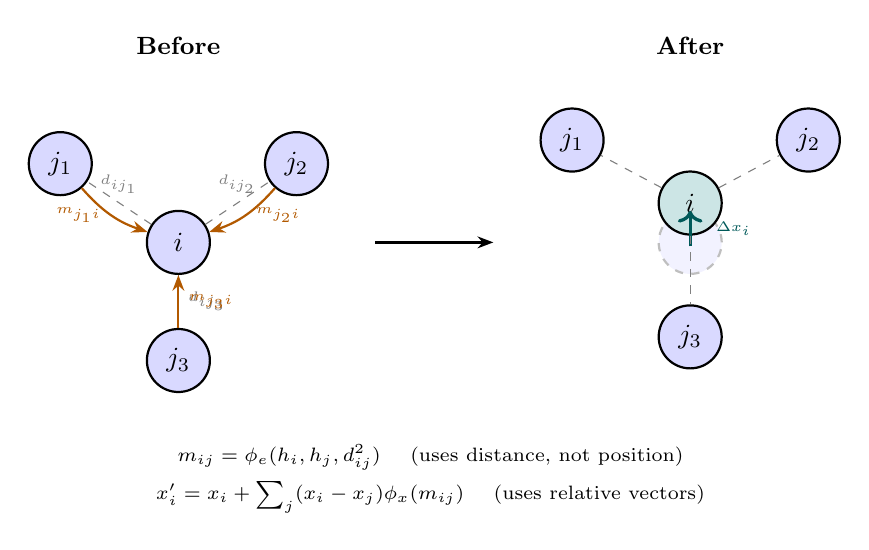
\begin{tikzpicture}[
    node distance=1.2cm,
    atom/.style={circle, draw, minimum size=0.8cm, thick, fill=blue!15},
    arrow/.style={-{Stealth[length=2mm]}, thick},
    msg/.style={-{Stealth[length=2mm]}, thick, orange!70!black},
    coord/.style={-{Stealth[length=2mm]}, very thick, teal!70!black},
    label/.style={font=\scriptsize},
    eqlabel/.style={font=\scriptsize, align=left}
]

% Left side: before update
\node[font=\small\bfseries] at (0, 2.5) {Before};

\node[atom] (i) at (0, 0) {$i$};
\node[atom] (j1) at (-1.5, 1) {$j_1$};
\node[atom] (j2) at (1.5, 1) {$j_2$};
\node[atom] (j3) at (0, -1.5) {$j_3$};

% Distance annotations
\draw[gray, dashed] (i) -- node[above, font=\tiny] {$d_{ij_1}$} (j1);
\draw[gray, dashed] (i) -- node[above, font=\tiny] {$d_{ij_2}$} (j2);
\draw[gray, dashed] (i) -- node[right, font=\tiny] {$d_{ij_3}$} (j3);

% Messages coming in
\draw[msg, bend right=15] (j1) to node[left, font=\tiny] {$m_{j_1i}$} (i);
\draw[msg, bend left=15] (j2) to node[right, font=\tiny] {$m_{j_2i}$} (i);
\draw[msg] (j3) to node[right, font=\tiny] {$m_{j_3i}$} (i);

% Arrow to right side
\draw[arrow, very thick] (2.5, 0) -- (4, 0);

% Right side: after update
\node[font=\small\bfseries] at (6.5, 2.5) {After};

% Ghost of original position
\node[atom, fill=blue!5, draw=gray!50, dashed] (i2ghost) at (6.5, 0) {};
\node[atom, fill=teal!20] (i2) at (6.5, 0.5) {$i$};
\node[atom] (j12) at (5, 1.3) {$j_1$};
\node[atom] (j22) at (8, 1.3) {$j_2$};
\node[atom] (j32) at (6.5, -1.2) {$j_3$};

% Arrow showing displacement
\draw[coord, ->] (6.5, -0.05) -- (6.5, 0.4);
\node[font=\tiny, teal!70!black] at (7.05, 0.17) {$\Delta x_i$};

% Connections
\draw[gray, dashed] (i2) -- (j12);
\draw[gray, dashed] (i2) -- (j22);
\draw[gray, dashed] (i2) -- (j32);

% Equations below
\node[eqlabel] at (3.25, -3) {
\begin{minipage}{7cm}
\centering
\scriptsize
$m_{ij} = \phi_e(h_i, h_j, d_{ij}^2)$ \quad (uses distance, not position)\\[3pt]
$x_i' = x_i + \sum_j (x_i - x_j) \phi_x(m_{ij})$ \quad (uses relative vectors)
\end{minipage}
};

\end{tikzpicture}

\caption{EGNN message passing. Scalar messages depend only on distances (rotation-invariant). Coordinate updates use relative position vectors $(x_i - x_j)$, which rotate with the input. The combination ensures the network is E(3)-equivariant.}
\label{fig:egnn}
\end{figure}

\begin{sciencebox}[Beyond vectors: spherical harmonics]
Scalars and vectors aren't the only geometric objects. Think about what happens when you rotate the coordinate system:
\begin{itemize}
\item A \textbf{scalar} (like energy) doesn't change at all.
\item A \textbf{vector} (like a force) rotates with the coordinates---its three components mix together according to the rotation matrix $R$.
\item A \textbf{quadrupole} (like the moment of inertia tensor) transforms in a more complicated way---it has five independent components that mix under rotation.
\end{itemize}
This pattern continues: there's a hierarchy of geometric objects labeled by $\ell = 0, 1, 2, \ldots$, with $2\ell + 1$ components each. These are the \emph{irreducible representations} of the rotation group.

\textbf{Spherical harmonics} $Y_\ell^m(\hat{r})$ provide a concrete basis for each level. You may know them from quantum mechanics: $\ell = 0$ is an $s$-orbital (spherical), $\ell = 1$ gives $p$-orbitals (three lobes along $x$, $y$, $z$), $\ell = 2$ gives $d$-orbitals (five cloverleaf patterns), and so on. They form a complete basis for any angular pattern on a sphere.

More advanced equivariant networks---NequIP~\cite{batzner2022nequip}, MACE~\cite{batatia2022mace}, Allegro~\cite{musaelian2023allegro}---represent features as collections of spherical harmonic components at each atom. The key operation is the \emph{tensor product}: combining two spherical harmonic features (say, $\ell = 1$ and $\ell = 1$) produces features at multiple orders ($\ell = 0, 1, 2$). The coefficients governing this combination are called \emph{Clebsch-Gordan coefficients}---fixed numbers from representation theory, not learned parameters.

The payoff is these networks capture directional interactions that scalar/vector architectures miss, like the angular dependence of chemical bonds or the anisotropy of crystal environments. The cost: mathematical and computational complexity. For a comprehensive introduction, see~\cite{duval2023hitchhiker}.
\end{sciencebox}

%%%%%%%%%%%%%%%%%%%%%%%%%%%%%%%%%%%%%%%%%%%%%%%%%%%%%%%%%%%%%%%%%%
\section{Forces from energy: equivariance for free}
%%%%%%%%%%%%%%%%%%%%%%%%%%%%%%%%%%%%%%%%%%%%%%%%%%%%%%%%%%%%%%%%%%

Suppose you train an invariant network to predict energy $E(\{x_i\})$. The forces are gradients:
\beq
F_i = -\nabla_{x_i} E
\eeq

If $E$ is rotation-invariant, then $F_i$ is automatically rotation-equivariant.

Working through it: Let $R$ be a rotation matrix. Invariance means $E(R\{x_i\}) = E(\{x_i\})$. Differentiate both sides with respect to $x_i$:
\beq
R^\top \nabla_{Rx_i} E = \nabla_{x_i} E
\eeq
So $\nabla_{Rx_i} E = R \nabla_{x_i} E$. The gradient at the rotated position equals the rotated gradient at the original position. That's equivariance.

The practical payof is that we can train a simple invariant network on energies and get forces for free by automatic differentiation. The forces are then exactly equivariant. This is how most modern machine learning potentials work: learn $E$, differentiate to get $F$, run molecular dynamics.
%
More generally: \textbf{symmetries of a function imply symmetries of its derivatives}. Build invariance into your energy predictor, and equivariance of forces follows automatically.

%%%%%%%%%%%%%%%%%%%%%%%%%%%%%%%%%%%%%%%%%%%%%%%%%%%%%%%%%%%%%%%%%%
\section{Why encode symmetry?}
%%%%%%%%%%%%%%%%%%%%%%%%%%%%%%%%%%%%%%%%%%%%%%%%%%%%%%%%%%%%%%%%%%

Why go through the trouble of building symmetry into architectures? After all, neural networks are universal approximators---with enough data, shouldn't they learn any symmetry implicitly? The advantage of encoding symmetry is largest with smaller datasets (less data to learn the symmetry implicitly), larger symmetry groups (more transformations to cover by augmentation), and stricter symmetry requirements (when approximate invariance isn't good enough---e.g., forces must be exactly equivariant for stable molecular dynamics).

\paragraph{Data augmentation: the alternative.} Instead of encoding symmetry in the architecture, we can \emph{augment} the training data: for each molecule, include rotated copies. The network sees all orientations and (hopefully) learns that orientation doesn't matter.

This works, but has costs---training on $N$ rotations multiplies compute by $N$. The network learns \emph{approximate} invariance---close to exact, but not perfect.

\paragraph{Data efficiency.} An equivariant network doesn't need to see every rotation of every molecule---it \emph{knows} that rotations preserve energy. A standard network must learn this from augmented data, requiring many more examples. When labeled data is scarce (common in science, where each label may require expensive simulations or experiments), equivariance can be the difference between a useful model and an overfit one.

Figure~\ref{fig:data_efficiency} illustrated this: equivariant networks (using higher-order spherical harmonic features, $L \geq 1$) achieve lower error at every training set size, with steeper improvement as data increases (more favorable scaling).

\begin{figure}[h]
\centering
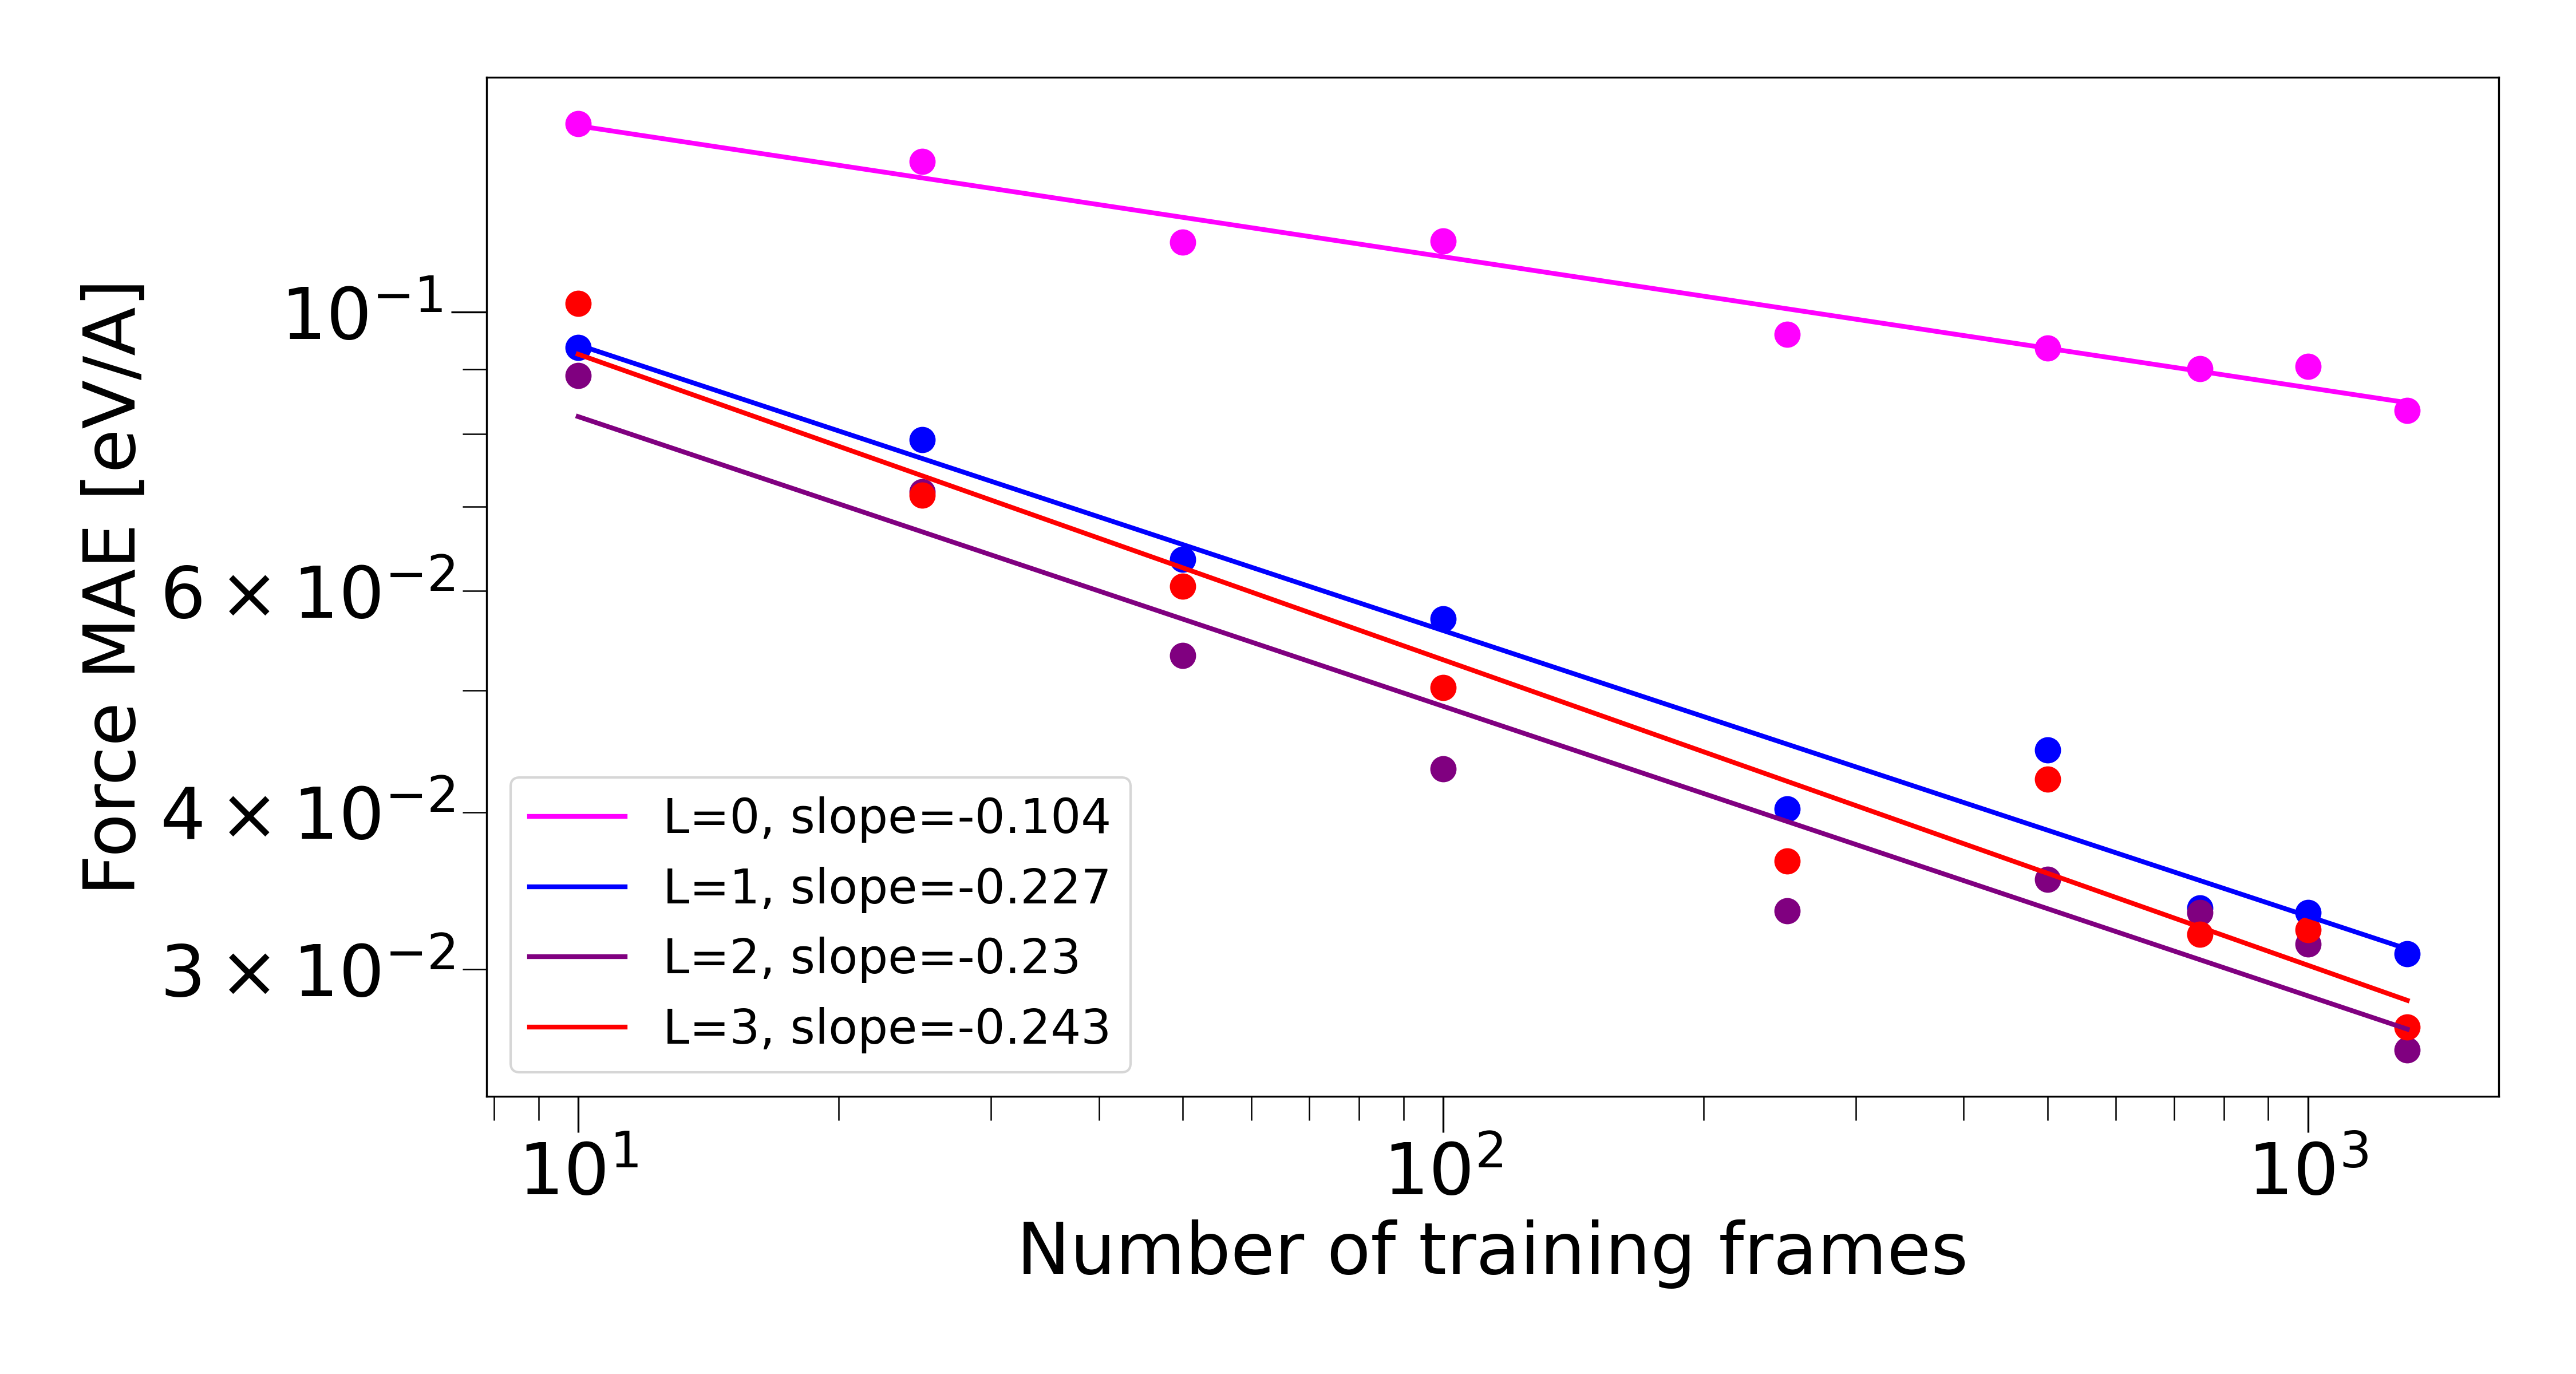
\includegraphics[width=0.7\textwidth]{figures/new_water_f_mae_data_eff.png}
\caption{Data efficiency of equivariant networks. Force prediction error vs.\ training set size for water molecules. $L=0$ uses only scalars (invariant); $L \geq 1$ includes vector and higher-order equivariant features. Equivariant networks achieve lower error at all training set sizes. Figure from~\cite{batzner2022nequip}.}
\label{fig:data_efficiency}
\end{figure}

\paragraph{Can augmentation catch up?} With enough epochs, yes---but at a cost. Recent scaling studies~\cite{brehmer2025equivariance} show that training non-equivariant networks with data augmentation can eventually match equivariant performance, but only when training for many more epochs on the same data. In the small-data regime where you'd train for thousands of epochs anyway, augmentation closes the gap. In the large-data regime where each sample is seen only once or a few times, equivariant networks maintain their advantage.

\paragraph{Compute efficiency.} Even with infinite data, equivariant networks remain more efficient. At any fixed compute budget---measured in floating-point operations---equivariant models outperform non-equivariant ones trained with augmentation (Figure~\ref{fig:compute_scaling}). Both model classes follow power-law scaling: double your compute, and the loss decreases by a predictable factor. But equivariant models maintain a consistent advantage across all tested compute budgets---roughly a factor of two in this benchmark. The symmetry constraint focuses learning capacity on the degrees of freedom that matter, rather than wasting capacity re-learning that rotations preserve energy.

\begin{figure}[h]
\centering
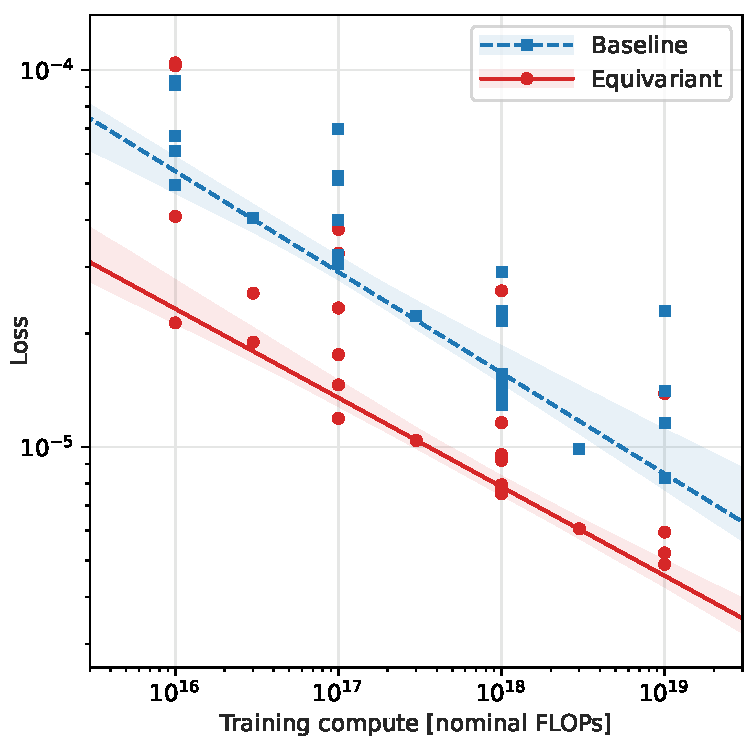
\includegraphics[width=0.55\textwidth]{figures/compute_scaling.pdf}
\caption{Compute scaling of equivariant vs.\ non-equivariant transformers on a rigid-body dynamics task. Both follow power-law scaling, but the equivariant model (red) consistently outperforms the non-equivariant baseline (blue) at every compute budget. The advantage persists even with large-scale training. Figure from~\cite{brehmer2025equivariance}.}
\label{fig:compute_scaling}
\end{figure}

\paragraph{When augmentation wins.} If the symmetry is only approximate, strict equivariance may be too strong. Images have gravity---up and down aren't equivalent. Molecules in solvent or on surfaces break full rotation symmetry. In these cases, learning an approximate symmetry from data may be more appropriate than enforcing an exact one. Augmentation also applies to any architecture without redesigning the model, which matters when leveraging pretrained models or established codebases.

\paragraph{Equivariance as a building block.} The architectures in this chapter are not standalone models but composable components. Diffusion models for molecules use equivariant score networks to ensure the learned distribution respects rotational symmetry. Machine learning potentials use equivariant networks to predict forces that transform correctly---critical for conserving angular momentum in long simulations. The design principles transfer beyond molecules to any domain with geometric structure: point clouds, meshes, robotics, physical simulations.

\bibliography{references}

\end{document}
